\chapter{Theoretical Framework II: Array-Level Optics}
\label{ch:array-theory}

\section{Mathematical array representation}
\label{sec:array-repr}
An array design is fully specified by: a \emph{family} (the geometric rule generating
hole center positions $\{(x_i,y_i)\}$), a hole diameter $a_{\mathrm{hole}}$ (identical
for every hole in a given design), a requested hole count $N$, and family-specific
spacing parameters (e.g.\ pitch and rotation for a lattice family, ring spacing and
holes-per-ring for a ring family). Eleven families are implemented in this project's
generator library (\texttt{Array\_Design/array\_geometry\_lab/array\_calculation/generators/},
verified via directory listing): \texttt{square}, \texttt{hexagonal},
\texttt{rectangular}, \texttt{concentric}, \texttt{concentric\_centered},
\texttt{ring\_offset\_concentric}, \texttt{archimedean\_spiral},
\texttt{fibonacci\_spiral}, \texttt{golden\_angle}, \texttt{poisson\_disk}, and
\texttt{jittered\_lattice}. Every generator recenters its own output on its own
centroid before returning coordinates (\texttt{base\_generator.py}, shared step), so
every design is symmetric about the array's own optical axis by construction.

For a square lattice with pitch $p$ and rotation $\theta_0$:
\begin{equation}
(x_i,y_i) = R(\theta_0)\cdot p\,(m,n), \qquad (m,n)\in\mathbb{Z}^2
\end{equation}
For a hexagonal lattice with the same pitch $p$ (nearest-neighbor spacing):
\begin{equation}
(x_i,y_i) = R(\theta_0)\cdot p\left(m + \tfrac12 n,\ \tfrac{\sqrt3}{2}n\right),
\qquad (m,n)\in\mathbb{Z}^2
\end{equation}
Both are checked directly against their own regenerated coordinates in
Section~\ref{sec:hex-intuition} against real fabricated designs.

\section{Fill factor and brightness}
The array's fill factor (fraction of the frame area occupied by open aperture) is
$f = N\pi(a_{\mathrm{hole}}/2)^2 / A_{\mathrm{hull}}$, where $A_{\mathrm{hull}}$ is the
convex-hull area of the hole pattern. Because every real winning design in this project
(Chapters~\ref{ch:model-a}, \ref{ch:model-b}) operates with only one hole illuminated at
a time under normal (straight-ahead) gaze (Section~\ref{sec:array-vs-single}), the fill
factor is not itself a brightness constraint in the way it would be for a simple neutral
filter; it is a \emph{geometric} density constraint, trading off against the blind-
fraction risk of Section~\ref{sec:blinding} -- a sparser array is more likely to leave a
gaze direction with no active hole at all.

\section{Comprehensive ghosting theory}
\label{sec:ghosting-theory}

\subsection{The crude formula and why it was replaced}
An early criterion for this project treated adjacent holes at pitch $s$ as producing
retinal images separated by $\Delta r \approx s\,v_r/d_{\mathrm{gap}}$, and called a
design ``ghost-free'' whenever $\Delta r$ was smaller than the single-hole blur radius.
Checked against two real, sold multi-pinhole eyewear patents (KR~10-2081511, pitch
3.2--4.8\,mm; CN~201716487U, pitch 0.7--1.2\,mm; both $d_{\mathrm{gap}}\approx12$\,mm),
this formula predicted severe ($30\times$--$400\times$) violations for \emph{both}
sold, presumably-functional products -- the contradiction that motivated a full
re-derivation (source: \texttt{Array\_Design/ghosting/THEORY.md} Section~1, verified
read directly). The formula was subsequently found to be independently wrong on its own
terms (re-derivation, \texttt{THEORY.md}'s own addendum) and is used nowhere in this
paper's reported results; it is included here only as the historical motivation for the
derivation that follows.

\subsection{Multi-hole image formation}
Under ordinary incoherent daylight illumination, the mutual coherence between light
paths through macroscopically-separated holes is negligible (Goodman,
\emph{Statistical Optics}); \emph{intensities}, not fields, add. Each active hole
produces its own copy of the single-hole point spread function, shifted to its own
retinal position:
\begin{equation}
I_{\mathrm{retina}}(\mathbf{r}) = \sum_i I_{\mathrm{single}}(\mathbf{r}-\mathbf{r}_i)
= I_{\mathrm{single}}(\mathbf{r}) * \mathrm{Comb}_{\{\mathbf{r}_i\}}(\mathbf{r})
\label{eq:comb}
\end{equation}
i.e.\ the multi-hole retinal image is exactly the single-hole PSF convolved with a Dirac
comb (or, for a general non-lattice array, a general sum of shifted delta functions) at
the active holes' own retinal image positions.

\subsection{The Fourier consequence the crude formula omitted}
By the convolution theorem, Equation~\ref{eq:comb} in frequency space is a
\emph{product}:
\begin{equation}
\hat{I}_{\mathrm{retina}}(f) = \mathrm{MTF}(f)\cdot\hat{\mathrm{Comb}}_{1/\Delta r}(f)
\end{equation}
The periodic ripple's fundamental frequency $f_0=1/\Delta r$ is attenuated by the
single-hole MTF (already computed by this project's own ASM pipeline,
Chapter~\ref{ch:single}) at that same frequency. A dense array (small pitch $s$, large
$f_0$) pushes the ghosting ripple's fundamental past the frequency where the MTF has
already rolled off toward zero -- multiple shifted copies smooth into one continuous
blur regardless of how large the raw pitch-vs-blur-radius ratio of the crude formula
would suggest. This is the central reason the crude formula was wrong for \emph{dense}
designs: it never accounted for the single-hole MTF's own low-pass character at all.

\subsection{The discrete precondition}
If the number of simultaneously-active holes $N_{\mathrm{eff}}\le1$ for a given pupil
alignment, there is only one term in the sum of Equation~\ref{eq:comb} -- no periodic
structure exists to be attenuated or perceived, regardless of pitch. This is the
\emph{active-pairs} mechanism this project's \texttt{margins/active\_pairs.py} and the
ghost gates of Chapter~\ref{ch:model-a} implement directly, and explains why a
sufficiently sparse array (e.g.\ the KR patent's own pitch) rarely ghosts even though
its raw pitch would fail the crude formula badly: most of the time, no second hole is
simultaneously active to ghost against at all.

\subsection{A refined three-regime criterion}
\label{sec:three-regime}
Combining the two mechanisms above, this project's synthesized ghosting-perceptibility
criterion is:
\begin{equation}
\text{Imperceptible if} \quad
N_{\mathrm{eff}}^{\mathrm{(worst\text{-}case)}}\le1 \quad \text{(Regime A)}
\qquad\text{OR}\qquad
\mathrm{MTF}(f_0) < \mathrm{CSF}^{-1}(f_0) \quad \text{(Regime B)}
\label{eq:three-regime}
\end{equation}
Regime C -- intermediate pitch, $N_{\mathrm{eff}}$ small but $>1$, and $f_0$ not yet
high enough for the MTF roll-off to suppress it below the CSF threshold -- is the
predicted \emph{danger zone}: a candidate physical mechanism for the double/triple-vision
and honeycomb/grating symptoms Kim et al.\ (2017) \citep{kim2017} directly report in
real subjects wearing real multi-pinhole glasses (\emph{``discomfort from after-images
such as honeycomb images, horizontal grating, and double or triple vision''}, quoted
directly, significantly worse than for single-pinhole glasses in the same study) --
overturning an earlier framing of this project's own investigation, which had asked why
real sold products show no reported ghosting at all; they do.

\begin{figure}[htbp]
\centering
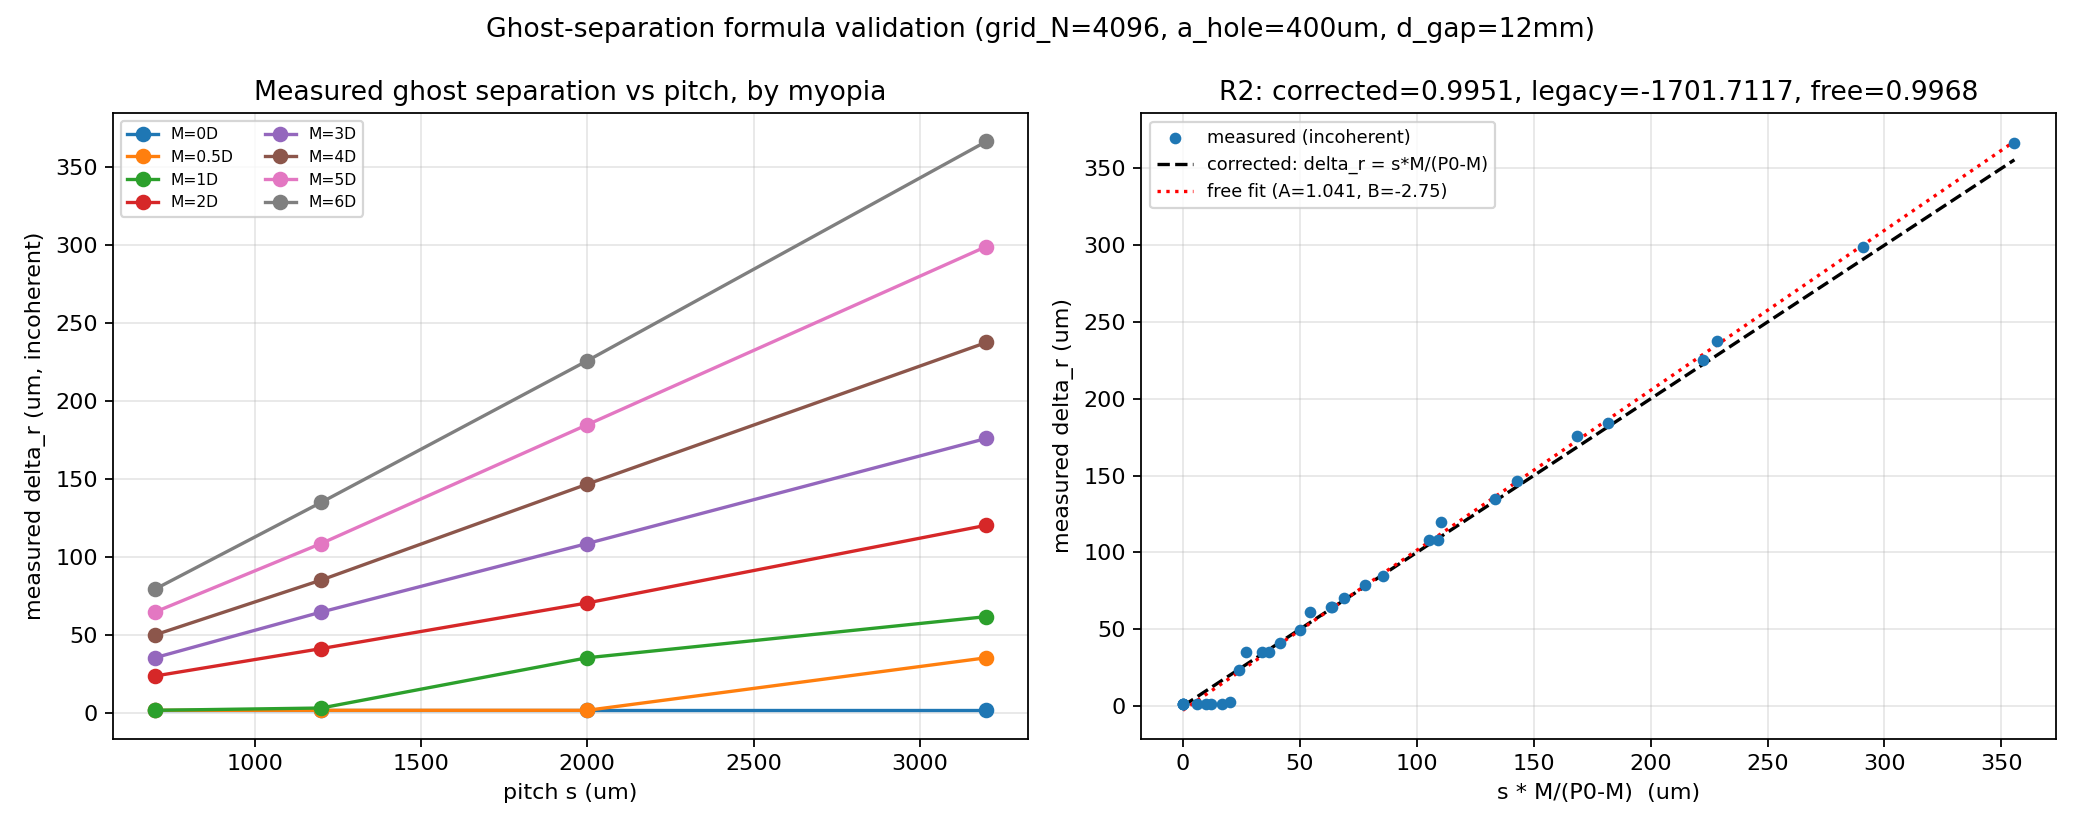
\includegraphics[width=\textwidth]{figures/ghost_formula_validation.png}
\caption{Independent validation of the ghost-separation formula
$\Delta r(s,M)=sM/(P_0-M)$ against measured (incoherent) two-hole separation from a
direct wave-optics simulation ($\mathtt{grid\_N}=4096$, $a_{\mathrm{hole}}=400\,\mu$m,
$d_{\mathrm{gap}}=12$\,mm), sweeping pitch $s$ at 8 myopia powers ($M=0$--$6$D). Right
panel: $R^2=0.9951$ for the corrected formula, versus $R^2=-1701.7$ for the legacy
formula this project explicitly disproved and stopped using (a negative $R^2$ --
worse than predicting the mean). A free 2-parameter affine fit recovers $A=1.041$,
$B=-2.75\,\mu$m, close to the zero-intercept unit-slope line the physics predicts.
Source: \texttt{Array\_Design/array\_optimization/stage0\_ghost\_validation/}
\texttt{ghost\_formula\_validation.png}, mtime 2026-08-14, the original validation run
this pipeline's own \texttt{engine/ghost\_formula.py} was copied from (byte-for-byte
verified against this same dataset, \texttt{VALIDATION.md}).}
\label{fig:ghost-validation}
\end{figure}

\section{The heuristic-CSF-out-of-range bug and the Barten (1999) fix}
\label{sec:barten}
Evaluating Equation~\ref{eq:three-regime} requires a CSF model. This project's own
first-pass CSF implementation (\texttt{Array\_Design/ghosting/contrast.py}) is a
heuristic, peak-matched to reported CSF peaks at 4--8\,cycles/degree (cpd), and was
\textbf{never fit or validated below its own peak frequency}.

\begin{warnbox}{Pass 1: a physically impossible result, traced to its root cause}
A 36-point sweep (apertures $\{300,400,700,1000\}\,\mu$m $\times$ pitches
$\{700,900,1200,1500,2000,2500,3200,4000,4800\}\,\mu$m, $M=4$D,
$d_{\mathrm{gap}}=12$\,mm, $\lambda=550$\,nm, $D_{\mathrm{pupil}}=4000\,\mu$m,
$N_{\mathrm{grid}}=1024$, square packing) found \textbf{zero} Regime~C points -- every
point classified as A (16/36) or B (20/36), i.e.\ every dense, potentially-dangerous
pitch was classified ``safe.'' Traced to root cause: every Regime-B point had a genuine
ghosting fundamental frequency $f_0<0.3$\,cpd (physically correct -- a near-eye,
millimetre-scale pitch genuinely produces a coarse, sub-1-cpd periodic pattern),
evaluated against the heuristic CSF model \emph{far outside its own fitted range}, which
in that regime returned a physically impossible required-contrast threshold of
16{,}337 to 1{,}000{,}000 (i.e.\ more than 100\% contrast) -- trivially satisfying
Regime~B (``safe'') regardless of the design's real MTF value. Source:
\texttt{Array\_Design/ghosting/RESULTS.md}, ``Pass 1'' section, verified read directly.
\end{warnbox}

\textbf{Fix:} a working implementation of the real Barten (1999) contrast sensitivity
model \citep{barten1999,barten2003} (simplified form via the published
\texttt{colour-science} Python package) was located and verified, with a stated valid
range of 0.2--50\,cpd -- overlapping this project's actual ghosting frequencies
(0.10--0.30\,cpd), unlike the heuristic. Sanity-checked first (threshold 0.6\%--3.6\%
across a 2--60\textdegree{} field-size range at that frequency, near-luminance-independent
-- physically sane behaviour, unlike the heuristic's out-of-range artifact).

\begin{center}
\begin{tabular}{lcc}
\toprule
Regime & Pass 1 (heuristic CSF) & Pass 2 (real Barten CSF) \\
\midrule
A (sparse, $N_{\mathrm{eff}}\le1$) & 16 & 16 (unchanged) \\
B (dense, CSF says safe) & 20 & \textbf{0} \\
C (danger zone) & 0 & \textbf{20} \\
\bottomrule
\end{tabular}
\end{center}
\textbf{Every previously-``safe'' dense point was reclassified as danger zone --
including the entire tested real dense-patent pitch range (700--1200\,$\mu$m).} This
reclassification is directionally consistent with Kim et al.\ (2017)'s directly-quoted
clinical finding above: the theory no longer needs an unresolved gap to explain that
finding away (source: \texttt{Array\_Design/ghosting/RESULTS.md}, ``Pass 2'').

\subsection{Pass 3: the harmonic series, not just the fundamental}
\label{sec:harmonic}
Passes 1--2 tested only the fundamental ghosting frequency $f_0=1/\Delta r$. A finite
train of $N$ shifted PSF copies (Equation~\ref{eq:comb}) is a genuinely periodic signal
with harmonic content at every $n f_0$ ($n=1,2,3,\dots$), not a single sinusoid.
Computing the full harmonic margin profile $\mathrm{MTF}(nf_0)/\mathrm{CSF}^{-1}(nf_0)$
for $n=1$ to $40$ at every dense-pitch test point found the worst-case harmonic is
\textbf{never} $n=1$: for the representative case $a_{\mathrm{hole}}=400\,\mu$m,
pitch $=900\,\mu$m, $M=4$D, the fundamental-alone margin is $75.6$ (already $>1$, i.e.\
already ``danger zone'' under Pass~2), but the actual worst harmonic is $n=9$, at
2.09\,cpd, with margin $329.2$ -- \textbf{4.4$\times$ more dangerous than the
fundamental alone predicted}.

\begin{keybox}{Why this generalizes, not just this one case}
MTF decreases smoothly and monotonically with frequency; the Barten CSF's own
sensitivity peak sits in a fixed \emph{absolute} frequency band ($\sim$2--5\,cpd)
regardless of pitch. The product of a monotonically-falling curve and a fixed-position
peak has its own peak at that same fixed absolute frequency -- changing the array pitch
only determines \emph{which harmonic index} $n$ happens to land near that peak, not
whether one does. Confirmed by re-running the full 36-point sweep with harmonic
analysis: the worst-case margin at a given aperture is essentially constant across
every dense pitch tested ($\sim329$ for $a_{\mathrm{hole}}=300$/$400\,\mu$m, $\sim273$
for $700\,\mu$m, $\sim219$ for $1000\,\mu$m), only the specific harmonic index achieving
it changes. Source: \texttt{Array\_Design/ghosting/RESULTS.md}, ``Pass 3.''
\end{keybox}

\section{Vignetting: gaze-dependent aperture activation}
\label{sec:vignetting}
As the wearer's eye rotates by eccentricity angle $\varphi$ from the array's own
optical axis, the pupil's center shifts laterally relative to the (head-fixed) array by
\begin{equation}
\Delta(\varphi) = R_{\mathrm{rot}}\sin\varphi
\label{eq:pupil-shift}
\end{equation}
with $R_{\mathrm{rot}}=13.5$\,mm (physiological range 13--14\,mm), in an azimuth
$\theta$ that can, physically, be any direction the wearer happens to look (source:
\texttt{Array\_Design/array\_geometry\_lab/array\_calculation/engine/vignetting\_overlap.py},
function \texttt{pupil\_shift\_um}, verified read directly). At each shifted pupil
position, the illuminated area contributed by hole $i$ (radius $R_h$) is the exact
circle--circle overlap area between the pupil disc (radius $R_p$) and that hole's disc,
handled in three explicit regimes with no implicit fallthrough:
\begin{equation}
A_{\mathrm{overlap}}(\Delta_i,R_p,R_h) =
\begin{cases}
\pi\min(R_p,R_h)^2 & \Delta_i \le |R_p-R_h| \quad \text{(full containment)} \\[4pt]
0 & \Delta_i \ge R_p+R_h \quad \text{(no overlap)} \\[6pt]
R_p^2\cos^{-1}\!\Big(\dfrac{\Delta_i^2+R_p^2-R_h^2}{2\Delta_i R_p}\Big)
+ R_h^2\cos^{-1}\!\Big(\dfrac{\Delta_i^2+R_h^2-R_p^2}{2\Delta_i R_h}\Big) & \\
\quad{}-\dfrac12\sqrt{(-\Delta_i+R_p+R_h)(\Delta_i+R_p-R_h)(\Delta_i+R_h-R_p)(\Delta_i+R_p+R_h)}
& \text{otherwise (partial overlap)}
\end{cases}
\label{eq:overlap}
\end{equation}
(Handbook 2, Sec.\ 13.2, implemented verbatim in \texttt{vignetting\_overlap.py}'s
\texttt{overlap\_area\_um2}, verified read directly.)

\begin{keybox}{A floating-point boundary defect, found and fixed}
Near the exact boundary $\Delta_i=R_p+R_h$, floating-point round-off on the two
$\cos^{-1}$ terms in the partial-overlap branch can produce a small \emph{negative}
computed area despite the true area being exactly zero there by construction --
observed concretely as $-0.0589\,\mu\mathrm{m}^2$ at $\Delta_i=3000\,\mu$m for a
$2000\,\mu$m hole. The implementation clamps the square-root term's radicand to
$[0,\infty)$ as a first safeguard, and clamps the final combined area to $[0,\infty)$ as
an independent second safeguard closing the same gap -- both present in the verified
current code, not merely proposed.
\end{keybox}

Independent validation: \texttt{vignetting\_overlap.py}'s copy of this formula (a
deliberate copy, not an import, so the array-geometry pipeline has zero runtime
dependency on the originating module's internals) was checked against its own
72-point validation dataset and reproduces it to \textbf{4.657$\times10^{-10}\,\mu$m$^2$
maximum absolute difference} (tolerance $10^{-6}\,\mu$m$^2$), with zero negative-area
outputs produced -- confirming the boundary-clamp fix was copied along with the formula,
not left behind (source: \texttt{VALIDATION.md}, verified present, this project's own
Part~1 validation gate).

\begin{figure}[htbp]
\centering
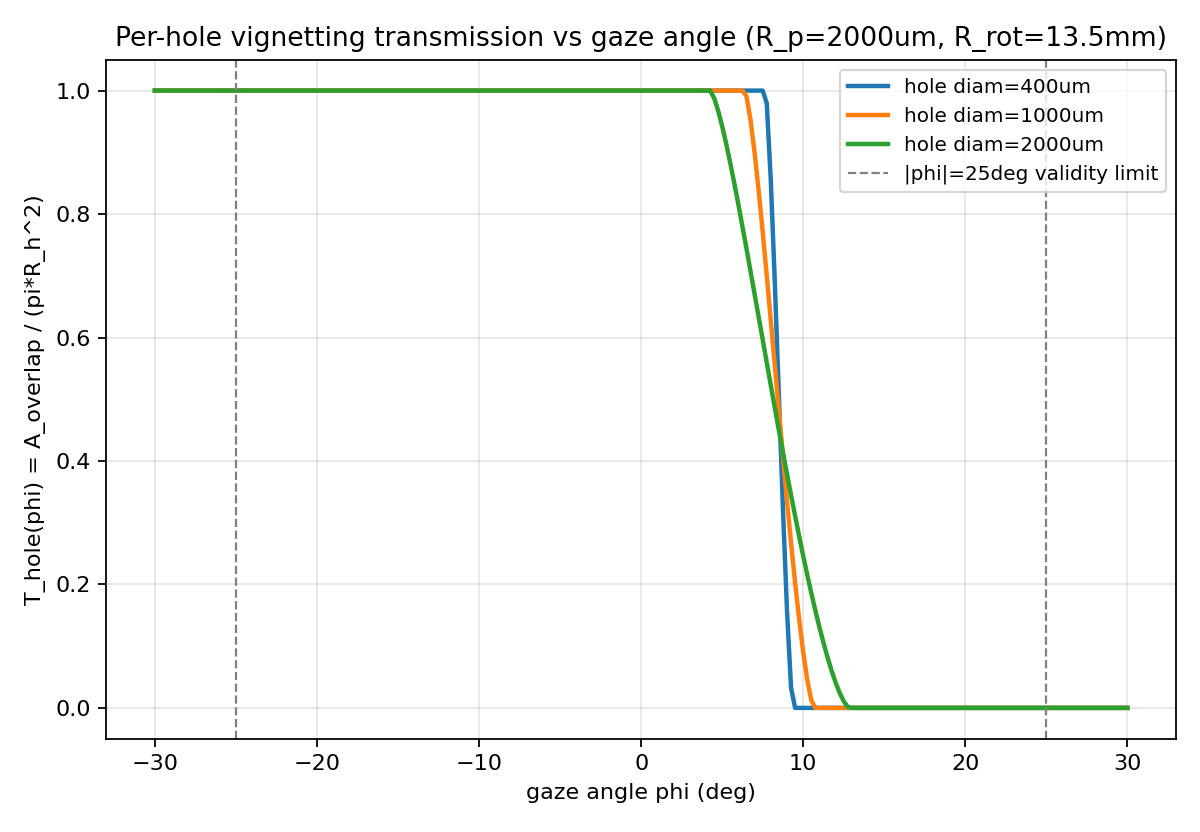
\includegraphics[width=0.75\textwidth]{figures/vignetting_validation.png}
\caption{Per-hole vignetting transmission $T_{\mathrm{hole}}(\varphi)=A_{\mathrm{overlap}}/(\pi
R_h^2)$ vs.\ gaze angle $\varphi$, three hole diameters, $R_p=2000\,\mu$m,
$R_{\mathrm{rot}}=13.5$\,mm. Transmission is exactly $1.0$ (full illumination) until
the pupil begins to slide off the hole, then falls to exactly $0.0$ over a narrow
angular transition -- the sharpness of this cutoff (a few degrees, not a gradual
taper) is what makes vignetting a genuine on/off hazard rather than a smooth
brightness gradient. The dashed vertical lines mark $|\varphi|=25^\circ$, this
formula's (Equation~\ref{eq:pupil-shift}) own stated small-angle validity limit --
Chapter~\ref{ch:model-b}'s $27^\circ$ extrapolated bin sits just outside it, flagged
there as extrapolated, not silently trusted. Source:
\texttt{Array\_Design/array\_optimization/vignetting\_validation.png}, mtime
2026-08-15, the original validation run \texttt{vignetting\_overlap.py} was copied
from.}
\label{fig:vignetting-transmission}
\end{figure}

\subsection{Single-axis vs.\ full-azimuth sampling}
\label{sec:single-axis-limitation}
This project's original vignetting evaluation (\texttt{margins/vignetting\_robustness.py})
models gaze along a \emph{single axis} only -- the pupil shifts to
$(\Delta(\varphi),0)$, never at any other azimuth $\theta$ -- matching the convention of
the module it was derived from. This is a real, acknowledged modelling limitation
(Section~\ref{sec:model-a-limitation}), not an oversight left undocumented: the module's
own docstring states plainly that this convention was inherited, and Model~B
(Chapter~\ref{ch:model-b}) was built specifically to remove it.

\section{Blinding, and the fundamental array trade-off}
\label{sec:blinding}
A gaze direction is \emph{blind} when the total illuminated area across every hole is
exactly zero: $\sum_i A_{\mathrm{overlap}}(\Delta_i(\varphi,\theta),R_p,R_h)=0$ -- no
light reaches the retina at that gaze direction at all, as distinct from a
\emph{ghosting} gaze direction, where two or more holes are simultaneously active
(quantified via the active-hole-fraction threshold of Section~\ref{sec:three-regime}).
These two failure modes trade directly against each other through the array's own
pitch: a denser array (smaller pitch, for a fixed hole size) is less likely to leave any
gaze direction blind, because some hole is more likely to be near the shifted pupil at
any given $(\varphi,\theta)$ -- but a denser array is, by the same token, more likely to
have \emph{two} holes simultaneously within the pupil at once, i.e.\ more likely to
ghost. This project's own real, already-computed data confirms this trade-off is not
merely theoretical: at matched pitch (4000\,$\mu$m, $M=2$D, $a_{\mathrm{hole}}=750\,\mu$m),
a ring-based design with 8 holes per ring achieves lower blind fraction (0.03\%) than
its 6-holes-per-ring counterpart (0.23\%) precisely by pulling ring holes closer
together angularly -- but pays for it with a real 7.58\% time-weighted ghost fraction,
against 0.00\% for the 6-hole variant (Section~\ref{sec:hex-intuition},
Figure~\ref{fig:geom-consequence}). Hexagonal packing is shown in
Chapter~\ref{ch:model-b} to be the one family tested that achieves near-zero on
\emph{both} metrics simultaneously at the same matched spacing, rather than trading one
against the other.
